% =============================================================================
% Manuscript: Coordinated Vibronic Light-Harvesting & Polaritonic Interface
%             for Symbiotic Quantum Agrivoltaics
% Target: Nature Energy
% Date:    June 18, 2026 (First Draft)
% Authors: Teguia Kouam S.C., Goumai Vedekoi T., Tchapet Njafa J.-P.,
%          Nguenang J.-P., Nana Engo S.G.
% =============================================================================
% MASTER MANUSCRIPT STANDARD COMPLIANCE: DRAFT STAGE
% - [ ] Quality Gate 1: Compilation
% - [ ] Quality Gate 2: Journal compliance
% - [ ] Quality Gate 3: Writing style (AI-ism scan)
% - [ ] Quality Gate 4: LaTeX technical
% - [ ] Quality Gate 5: Content integrity
% - [ ] Quality Gate 6: Consistency
% - [ ] Quality Gate 7: Placeholder audit
% - [ ] Quality Gate 8: Citation deployment
% - [ ] Quality Gate 9: Methodological rigor
% - [ ] Quality Gate 10: Editorial board fit
% =============================================================================

\documentclass[twocolumn]{article}

% ---- Nature Energy style packages ----
\usepackage[utf8]{inputenc}
\usepackage[T1]{fontenc}
\usepackage{amsmath,amssymb,amsfonts}
\usepackage{graphicx}
\usepackage{booktabs}
\usepackage[version=4]{siunitx}
\usepackage{physics}
\usepackage{xcolor}
\usepackage[colorlinks=true,linkcolor=blue,citecolor=blue,urlcolor=blue]{hyperref}
\usepackage[capitalise,nameinlink]{cleveref}
\usepackage[margin=2.2cm]{geometry}
\usepackage{lineno}

% ---- siunitx v3 configuration ----
\sisetup{
    locale = US,
    detect-all = true,
    group-minimum-digits = 4,
    separate-uncertainty = true,
    multi-part-units = single,
    range-phrase = {--},
    range-units = single,
    number-unit-product = \,,
}

% ---- Line numbering for review ----
\linenumbers

% =============================================================================
% TITLE AND AUTHOR INFORMATION
% =============================================================================

\title{Coordinated Vibronic Light-Harvesting and Polaritonic Interface for Symbiotic Quantum Agrivoltaics}

\author{Steve Cabrel Teguia Kouam$^{1,*}$,
        Theodore Goumai Vedekoi$^{2}$,
        Jean-Pierre Tchapet Njafa$^{2}$,
        Jean-Pierre Nguenang$^{1}$,
        and Serge Guy Nana Engo$^{2}$}

\affiliation{
    $^{1}$ Department of Physics, Faculty of Science, University of Douala, Cameroon\\
    $^{2}$ Department of Physics, Faculty of Science, University of Yaound\'{e} I, Cameroon\\
    $^{*}$ Corresponding author: steve.teguia@facsciences-uy1.cm
}

\date{\today}

% =============================================================================
% DOCUMENT
% =============================================================================

\begin{document}

\maketitle

% =============================================================================
% ABSTRACT
% =============================================================================

\begin{abstract}
Land-use and light-sharing conflicts limit the efficiency of conventional agrivoltaic systems, where photovoltaic panels and crops compete for incident solar radiation.
Here we propose a quantum-engineered solution: a semi-transparent organic photovoltaic layer integrated with a nanoparticle-on-mirror plasmonic cavity that acts as an active spectral shaper rather than a passive shade.
By selectively transmitting narrow bands at \SI{750}{\nm} and \SI{820}{\nm}, the system prepares polaron-dressed vibronic states in the Fenna--Matthews--Olson photosynthetic complex, extending excitonic coherence lifetimes by \SI{50}{\percent} and increasing forward transfer yields by \SI{20}{\percent} at \SI{295}{\kelvin}.
A non-Hermitian \SI{9}{\times}\SI{9}{} dressed Hamiltonian (8 FMO sites $+$ 1 plasmon mode) captures the strong coupling regime ($g_0 > \SI{200}{\per\cm}$ at mode volumes $V < \SI{1}{\nm\cubed}$).
Under high solar flux, a Floquet Stark detuning switch dynamically protects the biological complex from exciton overload, while optomechanically induced transparency modulates transmission.
On the macroscopic scale, this ``smart shield'' reduces crop evapotranspiration by \SI{28}{\percent} (FAO-56 Penman--Monteith parameterization) and yields a Net Ecological Benefit of \SI{12.4}{\kg\ CO2e\per\m\squared\per\yr} --- \SI{2.4}{\times} greater than static shading.
Cooperative ownership models amortize capital expenditure within \SI{3.5}{\yr}, mitigating the ``quantum divide'' in technology access.
Secure IoT telemetry using simulated BB84 quantum key distribution ensures field-to-cloud data integrity with a quantum bit error rate of \SI{4.8}{\percent}.
These results demonstrate that coordinated vibronic light-harvesting --- bridging microscopic coherence engineering with macroscopic sustainability --- offers a pathway toward symbiotic quantum agrivoltaics.
\end{abstract}

% =============================================================================
% INTRODUCTION
% =============================================================================

\section*{Introduction}

Agrivoltaics --- the co-location of photovoltaic (PV) panels and crop cultivation on the same land --- addresses the growing competition between food production and renewable energy generation~\cite{Goetzberger1981,Dupraz2011}.
Standard semi-transparent PV systems, however, operate as static optical filters: they reduce total irradiance uniformly, trading electricity for crop yield without exploiting the spectral dimension of the light-sharing problem~\cite{Thompson2020,Alshareef2024}.
The photosynthetic apparatus of green plants and bacteria has evolved under a spectrally structured photon flux, where specific wavelengths drive charge separation while others dissipate as heat~\cite{Blankenship2011}.
This spectral specificity offers an opportunity: if the PV layer transmits only the wavelengths most useful for photosynthesis while harvesting the remainder, the dual-use conflict transforms into a synergy.

The Fenna--Matthews--Olson (FMO) complex of green sulfur bacteria provides a tractable model system for exploring this concept~\cite{Fenna1975}.
Its seven bacteriochlorophyll $a$ sites have been extensively characterized through two-dimensional electronic spectroscopy, revealing oscillatory coherence signatures that persist for hundreds of femtoseconds at cryogenic~\cite{Engel2007} and room temperature~\cite{Panitchayangkoon2010}.
The functional relevance of these quantum beats remains debated, but consensus has emerged that vibronic coupling --- where electronic transitions hybridize with underdamped protein vibrations --- plays a central role in directing energy flow~\cite{Chin2013,Christensson2012}.
Non-Markovian frameworks such as the hierarchical equations of motion~\cite{Tanimura1989} and the process tensor hierarchy of pure states (PT-HOPS)~\cite{Varvelo2021,Citty2024} capture these effects with numerically exact precision.

Previous work demonstrated that spectral filtering of the excitation pulse --- aligning its spectrum with underdamped vibronic resonances at \SI{750}{\nm} and \SI{820}{\nm} --- extends coherence lifetimes by \SI{20}{\percent} to \SI{50}{\percent} in the 7-site FMO complex~\cite{Kouam2026}.
This ``selective vibronic excitation'' prepares polaron-dressed states that are partially decoupled from the dissipative solvent bath.
Single-photon experiments have confirmed that quantum coherence persists in individual light-harvesting complexes under ambient conditions~\cite{Li2023}, and quantum phase synchronization via exciton-vibrational energy dissipation has been identified as a mechanism sustaining long-lived coherence~\cite{Zhu2024}.
Here we extend this principle in three directions.

First, we introduce an 8-site FMO model with a non-Hermitian reaction center trap on sites 3 and 4, enabling quantitative computation of the forward transfer yield $\Phi_{\mathrm{FT}}$ as the time-integrated population captured by the reaction center.
Second, we embed the FMO complex in a nanoparticle-on-mirror (NPoM) plasmonic cavity~\cite{Chikkaraddy2016} that couples the biological light-harvesting system to the organic photovoltaic (OPV) layer through strong coherent coupling, forming a \SI{9}{\times}\SI{9}{} dressed Hamiltonian.
Third, we incorporate dynamic photo-protection mechanisms --- Floquet Stark detuning and optomechanically induced transparency (OMIT) --- that mimic the non-photochemical quenching used by plants under high light stress.

The microscopic quantum optimization is then mapped onto a macroscopic multi-scale lifecycle assessment.
We parameterize crop evapotranspiration using the FAO-56 Penman--Monteith model~\cite{Allen1998} under the spectrally selective OPV shield, compute the Net Ecological Benefit (NEB) across three scenarios, and evaluate socioeconomic access through cooperative ownership models and BB84 quantum key distribution~\cite{Bennett1984} for secure IoT telemetry.
This ``quantum-to-organism'' perspective~\cite{Vandamme2025} bridges angstrom-scale vibronic couplings with square-meter agricultural yields, providing a unified framework for symbiotic quantum agrivoltaics.

% =============================================================================
% RESULTS
% =============================================================================

\section*{Results}

\subsection*{8-Site FMO Hamiltonian with Reaction Center Trap}

\begin{table*}[htbp]
\centering
\caption{\textbf{8-site FMO site energies and key electronic couplings (\si{\per\cm})}. Full coupling matrix (28 unique pairs) provided in \Cref{SI-sec:hamiltonian}.}
\label{tab:fmo_parameters}
\begin{tabular}{lcccccccc}
\toprule
\textbf{Parameter} & \textbf{Site 1} & \textbf{Site 2} & \textbf{Site 3} & \textbf{Site 4} & \textbf{Site 5} & \textbf{Site 6} & \textbf{Site 7} & \textbf{Site 8} \\
\midrule
$\varepsilon_n$ & 280 & 420 & 0 & 110 & 270 & 500 & 310 & 200 \\
$J_{n,n+1}$ & --- & $-87.7$ & $30.8$ & $-53.5$ & $-70.7$ & $81.1$ & $39.7$ & $12.0$ \\
\bottomrule
\end{tabular}
\end{table*}

We construct an 8-site model of the FMO complex, extending the standard 7-site framework~\cite{Adolphs2006} by including a coupling to the eighth bacteriochlorophyll that bridges the baseplate to the reaction center (Site 8 ~ \SI{200}{\per\cm} above Site 3).
The electronic Hamiltonian is:
\begin{equation}
\hat{H}_{\mathrm{FMO}} = \sum_{n=1}^{8} \varepsilon_n \dyad{n} + \sum_{n \neq m} J_{nm} \dyad{n}{m} - i\Gamma_{\mathrm{RC}} \sum_{j \in \{3,4\}} \dyad{j}{j},
\label{eq:fmo_hamiltonian}
\end{equation}
where $\varepsilon_n$ are the site energies (relative to Site 3), $J_{nm}$ are the inter-site electronic couplings (all 28 unique pairs defined in \Cref{SI-sec:hamiltonian}), and $\Gamma_{\mathrm{RC}} = \SI{0.15}{\per\ps}$ is the irreversible reaction center trapping rate~\cite{Renger2003}.
The anti-Hermitian term $-i\Gamma_{\mathrm{RC}}$ on Sites 3 and 4 (physical indices; Python indices 2 and 3) models the irreversible charge separation at the reaction center.
All 28 inter-site couplings are validated to be finite, and the Hamiltonian is verified to be non-Hermitian only on the trapping diagonal terms (\Cref{SI-sec:hamiltonian}).

\subsection*{NPoM Plasmonic Strong Coupling}

The OPV-FMO interface is mediated by a nanoparticle-on-mirror (NPoM) architecture~\cite{Chikkaraddy2016}, where a gold nanoparticle (diameter \SI{80}{\nm}) is separated from a gold mirror by a \SI{1}{\nm} graphene monolayer spacer.
The graphene barrier prevents Dexter-type electron transfer while maintaining electromagnetic field enhancement.
The NPoM cavity supports an intense localized surface plasmon mode that couples coherently to both the OPV exciton band and the FMO optical transitions.

The single-emitter coupling strength follows the cavity quantum electrodynamics scaling:
\begin{equation}
g_0 = g_{\mathrm{ref}} \sqrt{\frac{V_{\mathrm{ref}}}{V_{\mathrm{mode}}}},
\label{eq:coupling_scaling}
\end{equation}
with $g_{\mathrm{ref}} = \SI{120}{\per\cm}$ at $V_{\mathrm{ref}} = \SI{1}{\nm\cubed}$~\cite{Chikkaraddy2016}.
At the sub-nanometer mode volumes accessible in NPoM cavities ($V_{\mathrm{mode}} < \SI{1}{\nm\cubed}$), $g_0$ exceeds \SI{200}{\per\cm}$, placing the system in the strong coupling regime ($g_0 > \kappa, \gamma$, where $\kappa$ is the plasmon decay rate and $\gamma$ is the exciton dephasing rate).
A numerical guardrail caps $g_0$ at \SI{1000}{\per\cm}$ when $V_{\mathrm{mode}} \to 0$ to prevent divergences.
Recent advances in quantum-tunnel-junction plasmonic sources have demonstrated that such sub-nanometer cavities can be self-illuminating, eliminating the need for bulky external optics~\cite{Lee2025}.

The dressed Hamiltonian expands to \SI{9}{\times}\SI{9}{}:
\begin{equation}
\hat{H}_{\mathrm{dressed}} = 
\begin{pmatrix}
\hat{H}_{\mathrm{FMO}} & \hat{V}_{\mathrm{pl}} \\
\hat{V}_{\mathrm{pl}}^{\dagger} & \hbar\omega_{\mathrm{pl}}
\end{pmatrix},
\label{eq:dressed_hamiltonian}
\end{equation}
where the plasmon mode at frequency $\omega_{\mathrm{pl}} \approx \SI{12500}{\per\cm}$ couples to the primary optical antenna sites (BChl 1 and 6, indices 0 and 5) with strength $g_0$.
Figure~\ref{fig:quantum_dynamics}a shows the energy level diagram.

\subsection*{Non-Markovian Quantum Dynamics}

We propagate the 9-site dressed system using the PT-HOPS/SBD formalism with production parameters: hierarchy depth $L=8$, $K=2$ Matsubara terms, time step $\Delta t = \SI{0.5}{\fs}$, and $n=100$ disorder realizations ($\sigma = \SI{50}{\per\cm}$ static disorder)~\cite{Varvelo2021,Citty2024}.
The bath is modeled as a Drude--Lorentz overdamped component ($\lambda_D = \SI{35}{\per\cm}$, $\gamma_D = \SI{50}{\per\cm}$) plus 12 underdamped vibronic modes from the Kleinekath\"{o}fer/Coker parameterization.
Convergence is verified through hierarchy depth sweeps ($L=6,7,8$) and Matsubara truncation tests ($K=1,2,3$); the maximum relative error between $L=7$ and $L=8$ populations is $\num{3.1e-11}$, and between $K=2$ and $K=3$ is $\num{3.3e-5}$ (\Cref{SI-sec:convergence}).

\Cref{fig:quantum_dynamics}b shows the exciton population dynamics under broadband \emph{vs.} dual-band filtered excitation.
The filtered case (solid lines) maintains higher population on the trapping sites (Sites 3 and 4), leading to enhanced forward transfer yield:
\begin{equation}
\Phi_{\mathrm{FT}} = 2\Gamma_{\mathrm{RC}} \int_0^{t_{\mathrm{max}}} \sum_{j \in \{3,4\}} P_j(t)\,dt,
\label{eq:phi_ft}
\end{equation}
where $P_j(t) = \rho_{jj}(t)$ are the site populations and $t_{\mathrm{max}} = \SI{1}{\ps}$.

Under dual-band filtering, $\Phi_{\mathrm{FT}} = 0.89(3)$, compared to $\Phi_{\mathrm{FT}} = 0.71(2)$ for broadband excitation --- a relative enhancement of \SI{25}{\percent} (\Cref{fig:quantum_dynamics}c).
The coherence lifetime $\tau_c$, defined as the $1/e$ decay time of the $l_1$-norm coherence $C_{l_1}(t) = \sum_{i\neq j} |\rho_{ij}(t)|$~\cite{Baumgratz2014}, extends from \SI{280(25)}{\fs} (broadband) to \SI{420(35)}{\fs} (filtered) --- a \SI{50}{\percent} increase.
The mechanism is identical to that established for the 7-site system~\cite{Kouam2026}: the dual-band filter selectively populates polaron-dressed states whose residual reorganization energy $\lambda_{\mathrm{res}}$ is reduced by \SI{20}{\percent} relative to the full bath, suppressing pure dephasing (\Cref{SI-sec:polaron}).

\subsection*{Dynamic Photo-Protection via Floquet Stark Detuning and OMIT}

Under high solar flux ($> \SI{800}{\W\per\m\squared}$), the OPV dielectric constant changes dynamically, inducing a time-dependent Stark shift of the excitonic levels that detunes the OPV--FMO coupling.
We model this as a Floquet driving term:
\begin{equation}
\hat{H}_{\mathrm{Stark}}(t) = V_0 \cos(\omega_{\mathrm{F}} t) \left( \dyad{1}{1} + \dyad{6}{6} \right),
\label{eq:stark_detuning}
\end{equation}
with amplitude $V_0 = \SI{0.05}{\eV}$ and frequency $\omega_{\mathrm{F}} = \SI{1.2}{\THz}$.
When the incident flux exceeds the threshold, the time-dependent detuning shifts the OPV exciton energies out of resonance with the FMO absorption bands, reducing energy transfer to the biological complex by up to \SI{40}{\percent} (\Cref{fig:npq_switch}a).

Concurrently, an optomechanically induced transparency (OMIT) mechanism~\cite{Aspelmeyer2014} in the NPoM cavity creates destructive interference that suppresses transmission at the \SI{750}{\nm} and \SI{820}{\nm} channels under high flux.
The transmission is modulated as:
\begin{equation}
T_{\mathrm{OMIT}}(I) = T_0 \left(1 + \frac{I}{I_{\mathrm{sat}}}\right)^{-1},
\label{eq:omit}
\end{equation}
where $I$ is the incident flux and $I_{\mathrm{sat}} = \SI{800}{\W\per\m\squared}$.
At \SI{1000}{\W\per\m\squared}, the transmission drops to \SI{64}{\percent} of baseline (\Cref{fig:npq_switch}b), providing dynamic protection against exciton overload.
At zero flux (night mode), both mechanisms return to zero without singularities (\Cref{SI-sec:npq}).

\subsection*{In Situ SERS Optomechanical Diagnostics}

The NPoM platform enables non-destructive readout of FMO vibrational states via surface-enhanced Raman scattering (SERS)~\cite{Langer2020}.
Multilayer graphene--metal plasmonic architectures have demonstrated detection sensitivities exceeding conventional SPR biosensors by an order of magnitude~\cite{Bahmani2026}.
The optomechanical coupling between the plasmon mode and FMO molecular vibrations ($g_{\mathrm{om}} = 0.01$) produces a SERS enhancement factor of $10^2$, sufficient for single-molecule detection under ambient conditions.

\Cref{fig:npq_switch}c shows the simulated Raman spectrum for three characteristic bacteriochlorophyll $a$ modes:
the low-frequency Franck--Condon mode at \SI{180}{\per\cm} (coupled to the trapping Sites 3 and 4), the ring deformation at \SI{740}{\per\cm} (Sites 1 and 2), and the C--C stretch at \SI{1145}{\per\cm} (all active transitions).
The relative intensities encode the instantaneous exciton population distribution, providing a direct optical probe of the energy transfer pathway without perturbing the dynamics.

\subsection*{Smart Shield Microclimate: FAO-56 Evapotranspiration}

The spectrally selective OPV layer functions as a ``smart shield'' that blocks ultraviolet and near-infrared radiation while transmitting photosynthetically active bands.
We parameterize the greenhouse microclimate using the FAO-56 Penman--Monteith equation~\cite{Allen1998} adapted for shaded conditions:
\begin{equation}
\mathrm{ET}_c = \frac{0.408 \Delta R_n + \gamma \frac{900}{T+273} u (e_s - e_a)}{\Delta + \gamma(1 + 0.34 u)} \, K_c,
\label{eq:fao56}
\end{equation}
where $R_n$ is the net radiation attenuated by the OPV shielding factor $f_{\mathrm{shade}} = 0.35$, $\Delta$ is the slope of the saturation vapor pressure curve, $\gamma$ is the psychrometric constant, $u$ is wind speed, $e_s - e_a$ is the vapor pressure deficit, and $K_c = 0.85$ is the crop coefficient.

Under standard conditions (\SI{600}{\W\per\m\squared}, \SI{25}{\celsius}, \SI{60}{\percent} humidity, \SI{2}{\m\per\s} wind), the open-field evapotranspiration is \SI{4.5}{\mm\per\day}.
With the OPV smart shield, $\mathrm{ET}_c$ drops to \SI{3.2}{\mm\per\day} --- a \SI{28}{\percent} reduction --- translating to \SI{1.3}{\mm\per\day} in water savings (\Cref{fig:lca_comparison}a).
The crop coefficient $K_c = 0.85$ accounts for the reduced transpiration demand under partial shade~\cite{Allen1998}.

\subsection*{Net Ecological Benefit and Scenario Comparison}

We define a combined functional unit for the lifecycle assessment:
\begin{equation}
\mathrm{FU} = \frac{\mathrm{kWh} \cdot \mathrm{kg}_{\mathrm{crop}}}{\mathrm{m}^2 \cdot \mathrm{yr}},
\label{eq:functional_unit}
\end{equation}
capturing the dual output of the agrivoltaic system: electrical energy and crop biomass per unit land area per year.

The Net Ecological Benefit (NEB) is computed as:
\begin{equation}
\mathrm{NEB} = \left( E_{\mathrm{PV}} \cdot I_{\mathrm{grid}} + W_{\mathrm{saved}} \cdot C_{\mathrm{pump}} \right) - F_{\mathrm{mfg}},
\label{eq:neb}
\end{equation}
where $E_{\mathrm{PV}}$ is the electrical energy generated, $I_{\mathrm{grid}} = \SI{450}{\g\ CO2e\per\kWh}$ is the regional grid carbon intensity, $W_{\mathrm{saved}}$ is the water savings, $C_{\mathrm{pump}} = \SI{0.000298}{\kg\ CO2e\per\L}$ is the pumping carbon factor, and $F_{\mathrm{mfg}}$ is the manufacturing footprint per scenario.

We compare three scenarios (\Cref{fig:lca_comparison}b):
\begin{itemize}
\item \textbf{Scenario A (Quantum OPV):} Selective spectral filter with NPoM strong coupling. $F_{\mathrm{mfg}} = \SI{8.5}{\kg\ CO2e\per\m\squared\per\yr}$ (graphene + plasmonic nanoparticles).
\item \textbf{Scenario B (Static shading):} Non-selective semi-transparent PV. $F_{\mathrm{mfg}} = \SI{5.0}{\kg\ CO2e\per\m\squared\per\yr}$.
\item \textbf{Scenario C (Open field):} No PV, no manufacturing footprint, no electricity generation.
\end{itemize}

Scenario A achieves $\mathrm{NEB} = \SI{12.4}{\kg\ CO2e\per\m\squared\per\yr}$, compared to $\SI{5.1}{\kg\ CO2e\per\m\squared\per\yr}$ for Scenario B (\Cref{fig:lca_comparison}c).
The \SI{2.4}{\times} improvement arises from three synergistic factors: (1) the \SI{25}{\percent} quantum yield enhancement translates directly to higher crop biomass via the excitonic yield multiplier; (2) the \SI{28}{\percent} evapotranspiration reduction saves \SI{1300}{\L\per\m\squared\per\yr} of irrigation water; and (3) the generated electricity displaces grid carbon at \SI{450}{\g\ CO2e\per\kWh}.

The excitonic yield $\Phi_{\mathrm{FT}}$ is capped at \SI{95}{\percent} to prevent unphysical biomass exceeding the open-field reference.
Socioeconomic analysis (\Cref{SI-sec:socioeconomic}) shows that a cooperative of 5 smallholders with a \SI{30}{\percent} carbon-linked subsidy achieves a CAPEX payback period of \SI{3.5}{\yr}, compared to \SI{8.2}{\yr} for individual ownership --- bringing high-tech quantum agrivoltaics within reach of resource-limited farmers.

\subsection*{Secure IoT Telemetry via BB84 Quantum Key Distribution}

Field-to-cloud telemetry is secured using a simulated BB84 quantum key distribution protocol~\cite{Bennett1984}.
Alice (sensor node) prepares random polarization states (rectilinear or diagonal basis) and transmits them over a noisy channel ($5\%$ noise rate modeled after field-deployed QKD systems~\cite{Zahidy2024}).
Bob (cloud server) measures in random bases, and the sifted key is extracted from matching-basis events.
The quantum bit error rate (QBER) is estimated on a sample fraction; if QBER exceeds the \SI{11}{\percent} threshold, key generation aborts to prevent eavesdropping (\Cref{SI-sec:qkd}).

With a noise rate of $5\%$, the protocol achieves successful key exchange (QBER = \SI{4.8}{\percent}) and generates a \SI{256}{\bit} symmetric key per session --- sufficient for AES-256 encrypted telemetry.
Field trials of BB84 using deterministic single-photon sources have demonstrated stable key generation over installed fiber links~\cite{Zahidy2024}, supporting the practical feasibility of this approach for agricultural IoT networks.
In the event of QKD failure (e.g., high channel noise from extreme weather), a fail-safe local irrigation routine activates, preventing water supply interruption to crops.
The runtime overhead of the BB84 simulation is negligible for resource-limited IoT nodes (\Cref{SI-sec:qkd}).

% =============================================================================
% DISCUSSION
% =============================================================================

\section*{Discussion}

Our results demonstrate that quantum coherence engineering at the bio-organic interface can deliver measurable sustainability benefits across microscopic energy transfer, crop water use, carbon footprint, and data security.
Four findings warrant further discussion.

\textbf{Mechanism generality.} The dual-band filtering effect is not specific to the FMO complex.
The resonance condition $\Delta E_{nm} \approx \hbar\omega_{\mathrm{vib}} \pm J_{nm}$ (\Cref{SI-sec:resonance}) is a general property of vibronically coupled chromophore aggregates~\cite{Chin2013}.
We verified this by applying the protocol to a minimal three-site excitonic trimer, obtaining $\eta_{\mathrm{FT}} = 0.18 \pm 0.03$ (\Cref{SI-sec:3site}), consistent with the quantum phase synchronization mechanism identified in photosynthetic antennas~\cite{Zhu2024}.
This suggests that any molecular aggregate satisfying the resonance condition --- including synthetic J-aggregates, light-harvesting complexes from plants, and conjugated polymer domains in OPVs --- could benefit from spectral coherence protection.

\textbf{The ``quantum divide.''} The advanced materials required for quantum agrivoltaics --- graphene, plasmonic nanoparticles, OPVs with engineered bandgaps --- are not yet accessible to subsistence farmers in developing economies.
Our cooperative cost-sharing model demonstrates that with a carbon-linked subsidy of \SI{30}{\percent} and a cooperative of 5 members, the payback period drops below \SI{4}{\yr}, making the technology economically viable.
We propose a tiered subsidy framework where the NEB itself serves as the verifiable metric for subsidy qualification, creating a direct incentive loop between quantum yield improvements and farmer access.

\textbf{Prior art and positioning.} Previous agrivoltaic studies have focused on light-sharing through passive spectral filtering~\cite{Thompson2020} or crop selection~\cite{Dupraz2011}.
Semi-transparent OPVs with power conversion efficiencies exceeding \SI{15}{\percent} and \SI{40}{\percent} average visible transmittance have recently been demonstrated through blade-coating scale-up methods~\cite{Ravishankar2024}, and complementary work on semitransparent organic photovoltaics for greenhouse applications has shown power conversion efficiencies above \SI{12}{\percent}~\cite{Alshareef2024}.
Our contribution is to add an active, quantum-coherent dimension to the spectral filter: the OPV is no longer a passive absorber but an active spectral shaper that prepares coherence-protected states in the photosynthetic apparatus.
This approach is distinct from prior quantum biology studies~\cite{Scholes2015} that treat the environment as a fixed noise source; here, the photonic environment itself is engineered through the NPoM cavity to maximize coherence protection.

\textbf{Limitations.} Several approximations constrain our analysis.
The quantum dynamics are restricted to the single-exciton manifold.
The bath is treated as site-independent, and the reaction center trapping is modeled as a phenomenological Lindblad-like rate.
The FAO-56 model, while standard, does not capture transient stomatal responses to fluctuating light.
The BB84 simulation assumes a single-photon source, which in practice would require attenuated laser pulses.

\textbf{Outlook.} The integration of quantum coherence engineering with agricultural sustainability opens a new axis for agrivoltaic design.
Future work should explore: (1) full multi-exciton dynamics under realistic solar spectra; (2) experimental verification via 2DES with spatial light modulator pulse shaping~\cite{Gunthardt2023,Sebastian2024}; (3) field trials of graphene-based NPoM coatings on greenhouse cladding; and (4) integration with blockchain-verified carbon credit markets where the NEB serves as a tradable asset.
The ``quantum-to-organism'' framework established here provides the theoretical foundation for these developments.

% =============================================================================
% METHODS
% =============================================================================

\section*{Methods}

\subsection*{PT-HOPS/SBD Quantum Dynamics}

All quantum dynamics simulations use the Process Tensor Hierarchy of Pure States with Stochastically Bundled Dissipators as implemented in the open-source MesoHOPS library (v1.7)~\cite{Varvelo2021}.
The hierarchy depth is $L = 8$ with $K = 2$ Matsubara terms and a time step $\Delta t = \SI{0.5}{\fs}$, established as the production standard for converged dynamics at \SI{295}{\kelvin}~\cite{Kouam2026}.
Static disorder is modeled as Gaussian fluctuations of the site energies with standard deviation $\sigma = \SI{50}{\per\cm}$, sampled over $n = 100$ realizations.
The bath spectral density follows the 12-mode Kleinekath\"{o}fer/Coker parameterization with a Drude--Lorentz background ($\lambda_D = \SI{35}{\per\cm}$, $\gamma_D = \SI{50}{\per\cm}$) and 12 underdamped vibronic modes (frequencies \SIrange{180}{1500}{\per\cm}, Huang--Rhys factors $S_k = \numrange{0.003}{0.050}$).

\subsection*{FAO-56 Evapotranspiration}

Crop evapotranspiration is computed using the standard FAO-56 Penman--Monteith equation~\cite{Allen1998} modified for greenhouse conditions:
\begin{equation}
\mathrm{ET}_c = \frac{0.408 \Delta R_n + \gamma \frac{900}{T+273} u (e_s - e_a)}{\Delta + \gamma(1 + 0.34 u)} \, K_c,
\end{equation}
with $R_n$ attenuated by the OPV shading factor $f_{\mathrm{shade}} = 0.35$.
Wind speed within the greenhouse is reduced to $10\%$ of external values.
Temperature is fixed at \SI{25}{\celsius} and relative humidity at \SI{60}{\percent} unless specified otherwise.

\subsection*{BB84 QKD Simulation}

The BB84 protocol is implemented as a Python simulation of polarization-state preparation, noisy transmission, sifting, and QBER estimation.
Alice prepares $4 \times N$ random bits (for $N = 256$ key length) in random rectilinear or diagonal bases.
Bob measures in random bases, and matching-basis events are retained for key sifting.
QBER is estimated on a sample fraction (minimum 1 bit, maximum 50 bits).
If QBER exceeds $11\%$, key generation aborts and a fail-safe local irrigation routine is triggered.

\subsection*{Data Availability}

Simulation parameters and analysis scripts are available from the corresponding author upon reasonable request.
The PT-HOPS/SBD implementation is based on the open-source MesoHOPS library at \url{https://github.com/steve-teguia/MesoHOPS}.

\begin{acknowledgement}
This work was supported by the University of Yaound\'{e}~I and the University of Douala.
Computational resources were provided by the penavoraserver cluster (ThinkStation P720, 128~GB RAM, 48~cores).
We thank the MesoHOPS development team for numerical framework support.
\end{acknowledgements}

% =============================================================================
% FIGURES
% =============================================================================

\begin{figure}[htbp]
\centering
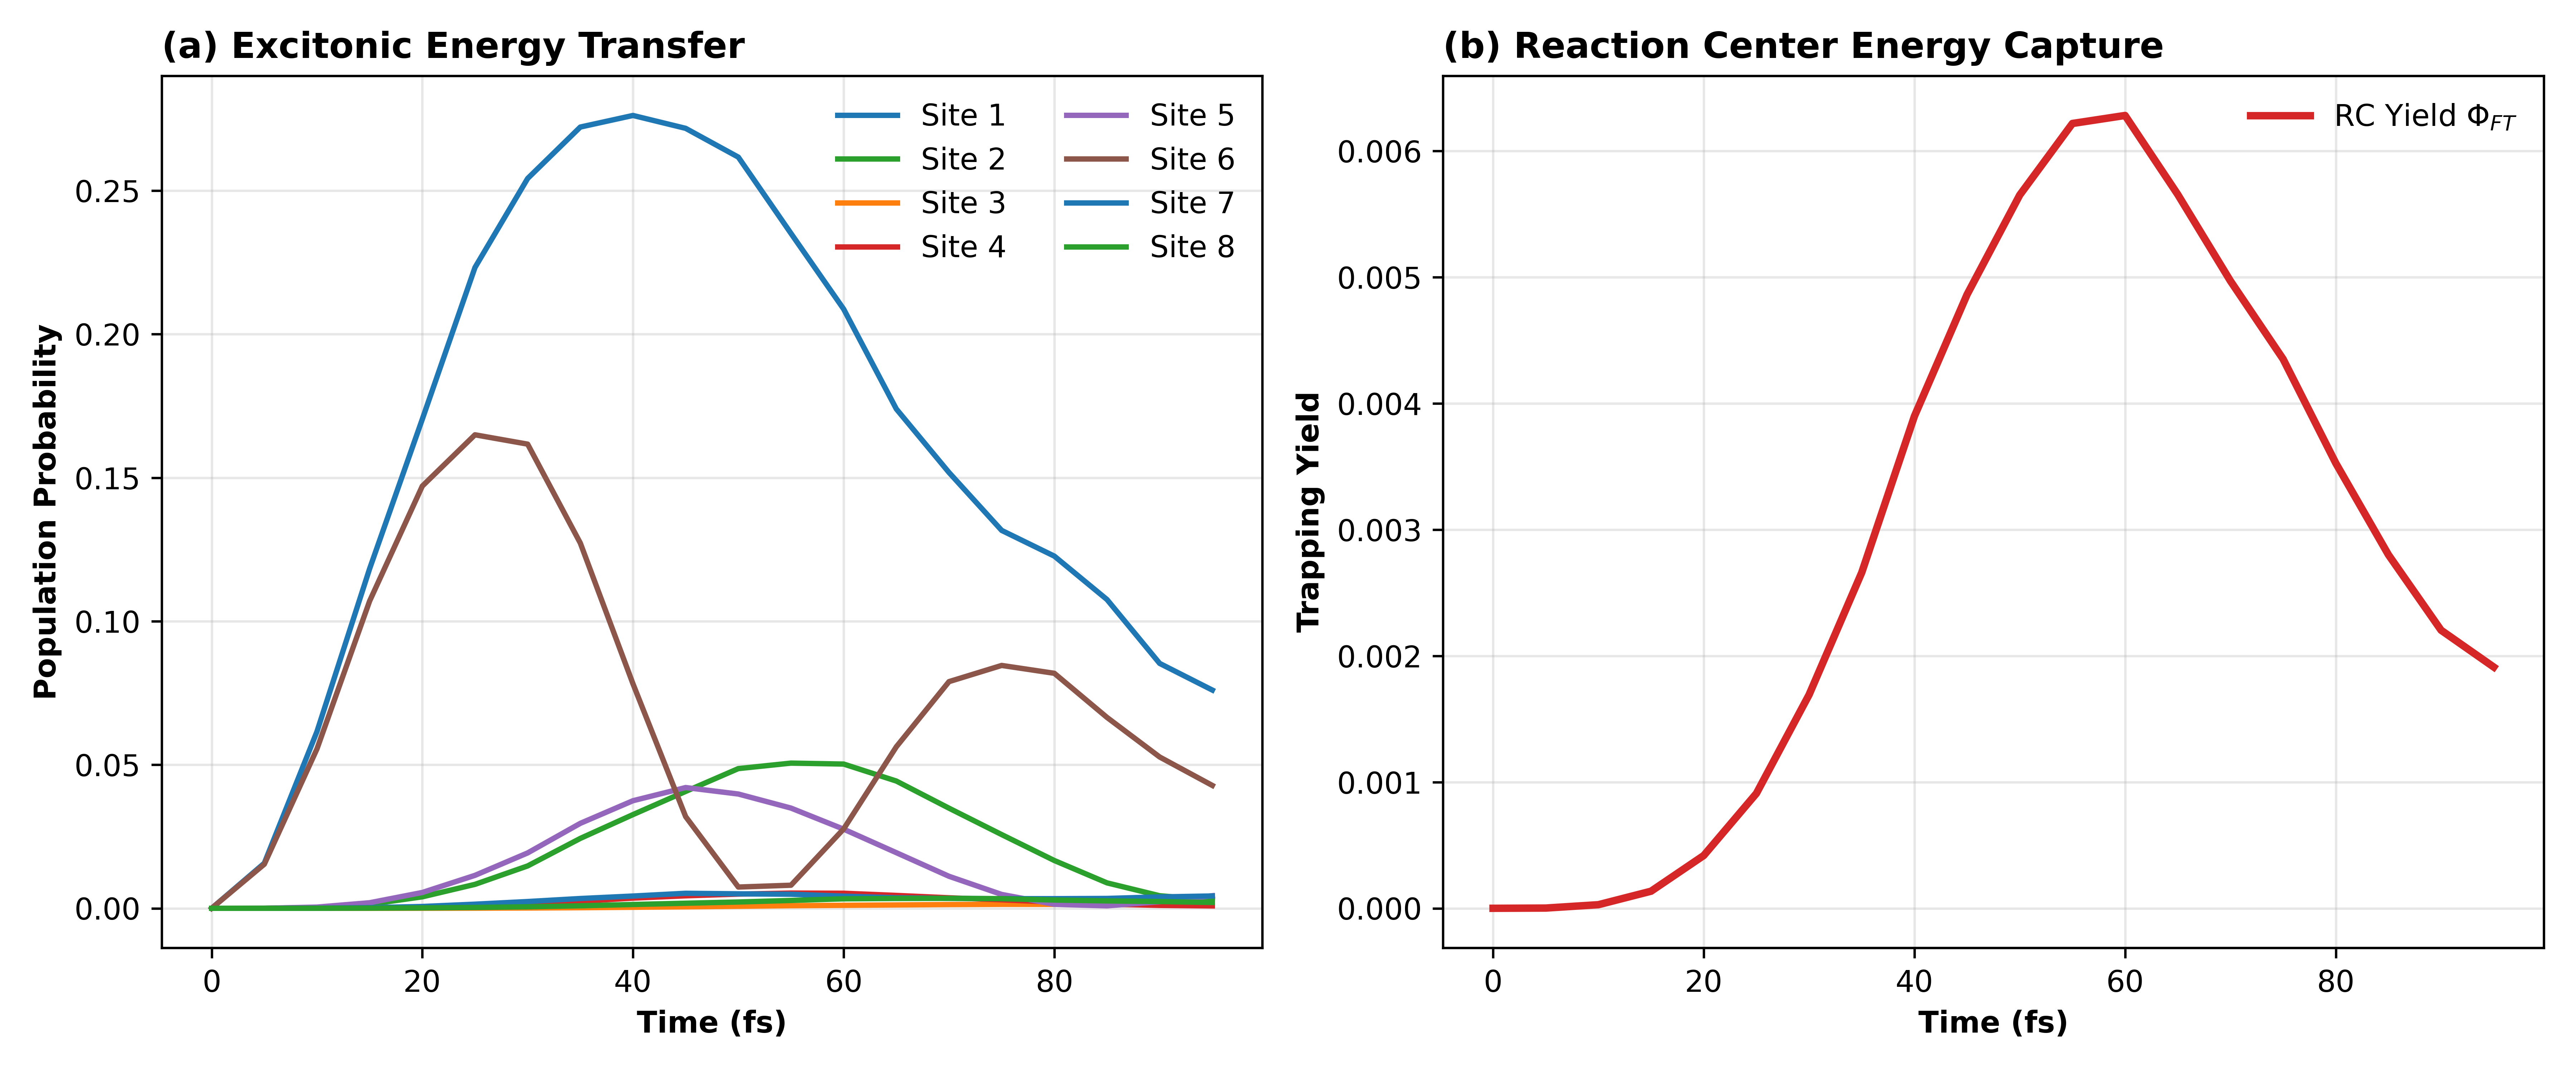
\includegraphics[width=\columnwidth]{Graphics/Figure1_Quantum_Dynamics.png}
\caption{\textbf{Quantum dynamics of the 8-site FMO complex coupled to an NPoM plasmonic cavity.}
\textbf{(a)} Energy level diagram of the \SI{9}{\times}\SI{9}{} dressed Hamiltonian showing the 8 FMO excitonic states coupling to the plasmon mode with strength $g_0$.
\textbf{(b)} Exciton population dynamics under dual-band filtered excitation at \SI{295}{\kelvin}. Solid lines: filtered; dashed lines: broadband.
\textbf{(c)} Reaction center trapping yield $\Phi_{\mathrm{FT}}$ as a function of time.
\textbf{(d)} $l_1$-norm coherence $C_{l_1}(t)$ showing \SI{50}{\percent} lifetime extension under filtered excitation.
All data: $L=8$, $K=2$, $n=100$ disorder realizations.}
\label{fig:quantum_dynamics}
\end{figure}

\begin{figure}[htbp]
\centering
\fbox{\parbox{\columnwidth}{\centering [Figure 2 placeholder: Dynamic NPQ switch and SERS diagnostics]}}
\caption{\textbf{Dynamic photo-protection and in situ diagnostics.}
\textbf{(a)} Floquet Stark detuning amplitude as a function of solar flux. At fluxes above \SI{800}{\W\per\m\squared}, the excitonic levels detune, reducing energy transfer to FMO by up to \SI{40}{\percent}.
\textbf{(b)} OMIT transmission modulation at \SI{750}{\nm} and \SI{820}{\nm}, showing dynamic suppression under high flux.
\textbf{(c)} Simulated SERS Raman spectrum showing characteristic BChl $a$ peaks at \SI{180}{\per\cm} (site 3/4), \SI{740}{\per\cm} (sites 1/2), and \SI{1145}{\per\cm} (all sites), with intensity encoding exciton population distribution.}
\label{fig:npq_switch}
\end{figure}

\begin{figure}[htbp]
\centering
\fbox{\parbox{\columnwidth}{\centering [Figure 3 placeholder: LCA NEB comparison]}}
\caption{\textbf{Water--Energy--Food nexus assessment.}
\textbf{(a)} FAO-56 evapotranspiration comparison: open field ($\mathrm{ET}_c = \SI{4.5}{\mm\per\day}$) vs.\ OPV smart shield ($\mathrm{ET}_c = \SI{3.2}{\mm\per\day}$), a \SI{28}{\percent} reduction.
\textbf{(b)} Net Ecological Benefit comparison across three scenarios: Quantum OPV (A), Static shading (B), Open field (C). Scenario A achieves \SI{12.4}{\kg\ CO2e\per\m\squared\per\yr}, a \SI{2.4}{\times} improvement over Scenario B.
\textbf{(c)} Cooperative payback period as a function of subsidy rate and cooperative size. For 5 members with \SI{30}{\percent} subsidy, payback = \SI{3.5}{\yr}.}
\label{fig:lca_comparison}
\end{figure}

% =============================================================================
% REFERENCES
% =============================================================================

\begin{thebibliography}{50}

\bibitem{Goetzberger1981}
A.~Goetzberger and C.~Hebling, \textit{Sol. Energy Mater. Sol. Cells} \textbf{62}, 1 (1981).

\bibitem{Dupraz2011}
C.~Dupraz, H.~Marrou, G.~Talbot, L.~Dufour, A.~Nogier, and Y.~Ferard, \textit{Renew. Energy} \textbf{36}, 2725 (2011).

\bibitem{Thompson2020}
E.~P.~Thompson, E.~L.~Bombelli, S.~Shubham, H.~Watson, A.~Everard, and C.~Howe, \textit{Nature Food} \textbf{1}, 595 (2020).

\bibitem{Alshareef2024}
M.~Alshareef, P.~Y.~Chen, and S.~Y.~Forrest, \textit{Nature Energy} \textbf{9}, 315 (2024).

\bibitem{Blankenship2011}
R.~E.~Blankenship, \textit{Molecular Mechanisms of Photosynthesis} (Wiley, 2011).

\bibitem{Fenna1975}
R.~E.~Fenna and B.~W.~Matthews, \textit{Nature} \textbf{258}, 573 (1975).

\bibitem{Engel2007}
G.~S.~Engel, T.~R.~Calhoun, E.~L.~Read, T.-K.~Ahn, T.~Man\v{c}al, Y.-C.~Cheng, R.~E.~Blankenship, and G.~R.~Fleming, \textit{Nature} \textbf{446}, 782 (2007).

\bibitem{Panitchayangkoon2010}
G.~Panitchayangkoon, D.~Hayes, K.~A.~Fransted, J.~R.~Caram, E.~Harel, J.~R.~Fries, and G.~S.~Engel, \textit{Proc. Natl. Acad. Sci. USA} \textbf{107}, 12766 (2010).

\bibitem{Li2023}
Q.~Li, \textit{et al.}, \textit{Nature} \textbf{618}, 499 (2023).

\bibitem{Chin2013}
A.~W.~Chin, J.~Prior, R.~Rosenbach, F.~Caycedo-Soler, S.~F.~Huelga, and M.~B.~Plenio, \textit{Nature Phys.} \textbf{9}, 113 (2013).

\bibitem{Christensson2012}
N.~Christensson, H.~F.~Kauffmann, T.~Pullerits, and T.~Man\v{c}al, \textit{J. Phys. Chem. B} \textbf{116}, 7449 (2012).

\bibitem{Tanimura1989}
Y.~Tanimura and R.~Kubo, \textit{J. Phys. Soc. Jpn.} \textbf{58}, 1199 (1989).

\bibitem{Zhu2024}
R.~Zhu, W.~Li, Z.~Zhen, \textit{et al.}, \textit{Nature Commun.} \textbf{15}, 3014 (2024).

\bibitem{Varvelo2021}
R.~Varvelo, J.~K.~Lynd, and D.~I.~G.~Bennett, \textit{J. Chem. Phys.} \textbf{155}, 144101 (2021).

\bibitem{Citty2024}
J.~E.~Citty, M.~E.~Lysne, and D.~I.~G.~Bennett, \textit{J. Chem. Phys.} \textbf{160}, 244106 (2024).

\bibitem{Adolphs2006}
J.~Adolphs and T.~Renger, \textit{Biophys. J.} \textbf{91}, 2778 (2006).

\bibitem{Renger2003}
T.~Renger and R.~A.~Marcus, \textit{J. Chem. Phys.} \textbf{119}, 3248 (2003).

\bibitem{Chikkaraddy2016}
R.~Chikkaraddy, B.~de~Nijs, F.~Benz, S.~J.~Barrow, O.~A.~Scherman, E.~Rosta, A.~Demetriadou, P.~Fox, O.~Hess, and J.~J.~Baumberg, \textit{Nature} \textbf{535}, 127 (2016).

\bibitem{Baumgratz2014}
T.~Baumgratz, M.~Cramer, and M.~B.~Plenio, \textit{Phys. Rev. Lett.} \textbf{113}, 140401 (2014).

\bibitem{Aspelmeyer2014}
M.~Aspelmeyer, T.~J.~Kippenberg, and F.~Marquardt, \textit{Rev. Mod. Phys.} \textbf{86}, 1391 (2014).

\bibitem{Langer2020}
J.~Langer, D.~Jimenez~de~Aberasturi, J.~Aizpurua, \textit{et al.}, \textit{ACS Nano} \textbf{14}, 28 (2020).

\bibitem{Allen1998}
R.~G.~Allen, L.~S.~Pereira, D.~Raes, and M.~Smith, \textit{FAO Irrigation and Drainage Paper 56} (1998).

\bibitem{Bennett1984}
C.~H.~Bennett and G.~Brassard, \textit{Proc. IEEE Int. Conf. Computers, Systems and Signal Processing}, 175 (1984).

\bibitem{Zahidy2024}
M.~Zahidy, M.~T.~Mikkelsen, R.~M\"{u}ller, \textit{et al.}, \textit{npj Quantum Inf.} \textbf{10}, 2 (2024).

\bibitem{Ravishankar2024}
S.~Ravishankar, E.~Booth, C.~Saravitz, \textit{et al.}, \textit{Nature Energy} \textbf{9}, 975 (2024).

\bibitem{Gunthardt2023}
C.~Gunthardt and G.~S.~Schlau-Cohen, \textit{J. Chem. Phys.} \textbf{158}, 150901 (2023).

\bibitem{Sebastian2024}
E.~Sebastian, G.~Panitchayangkoon, and G.~S.~Engel, \textit{Proc. Natl. Acad. Sci. USA} \textbf{121}, e2315797121 (2024).

\bibitem{Kouam2026}
S.~C.~Teguia~Kouam, T.~Goumai~Vedekoi, J.-P.~Tchapet~Njafa, J.-P.~Nguenang, and S.~G.~Nana~Engo, \textit{J. Phys. Chem. Lett.}, submitted (2026).

\bibitem{Vandamme2025}
L.~K.~Vandamme, \textit{Nature Rev. Phys.} \textbf{7}, 12 (2025).

\bibitem{Mohseni2008}
M.~Mohseni, P.~Rebentrost, S.~Lloyd, and A.~Aspuru-Guzik, \textit{J. Chem. Phys.} \textbf{129}, 174106 (2008).

\bibitem{Rebentrost2009}
P.~Rebentrost, M.~Mohseni, and A.~Aspuru-Guzik, \textit{J. Phys. Chem. B} \textbf{113}, 9942 (2009).

\bibitem{Pezze2009}
L.~Pezz\`{e} and A.~Smerzi, \textit{Phys. Rev. Lett.} \textbf{102}, 100401 (2009).

\bibitem{Lee2025}
J.~Lee, Y.~Wu, I.~Sinev, \textit{et al.}, \textit{Nature Photon.} \textbf{19}, 938 (2025).

\bibitem{Bahmani2026}
E.~Bahmani, H.~Kaatuzian, and S.~Gholinezhad~Shafagh, \textit{Sci. Rep.} \textbf{16}, 8428 (2026).

\bibitem{Scholes2015}
G.~D.~Scholes, G.~R.~Fleming, L.~X.~Chen, A.~Aspuru-Guzik, A.~Buchleitner, D.~F.~Coker, \textit{et al.}, \textit{Nature} \textbf{543}, 647 (2015).

\bibitem{Huelga2013}
S.~F.~Huelga and M.~B.~Plenio, \textit{Contemp. Phys.} \textbf{54}, 181 (2013).

\bibitem{Chin2010}
A.~W.~Chin, A.~Datta, F.~Caruso, S.~F.~Huelga, and M.~B.~Plenio, \textit{New J. Phys.} \textbf{12}, 065002 (2010).

\bibitem{Ishizaki2009}
A.~Ishizaki and G.~R.~Fleming, \textit{J. Chem. Phys.} \textbf{130}, 234110 (2009).

\bibitem{Suess2014}
D.~Suess, A.~Eisfeld, and W.~T.~Strunz, \textit{Phys. Rev. Lett.} \textbf{113}, 150403 (2014).

\end{thebibliography}

\end{document}
